\section{Finding equilibria and bounds on parameters}

Depending on the choice of parameters, there is either one (stable), two (stable-unstable) or three (stable-unstable-stable) equilibria to \ref{system}. In each scenario, the origin $(0, 0, 0)$ is a stable steady state. For a specific range of parameters, another stable, positive equilibrium arises whose value turns out to be rather cumbersome to compute due to the "Michaelis-Menten" term in the kinetics equations, see (\ref{fig:nullclines}). However, having in mind that the choice of parameters directly impacts the value of $\bar X$, one can derive a set of conditions $\bar X$ must satisfy in order for this positive steady-state to exists.

\begin{figure}[h]
	\floatbox[{\capbeside\thisfloatsetup{capbesideposition={left,center},capbesidewidth=0.5\linewidth}}]{figure}[1.2\FBwidth]
	{\caption{Algebraic curves describing the Nullclines of the system. in blue, $f^1(u, v, w) = 0$, green, $f^2(u, v, w) = 0$ and red, $f^3(u, v, w) = 0$ }\label{fig:nullclines}}
	{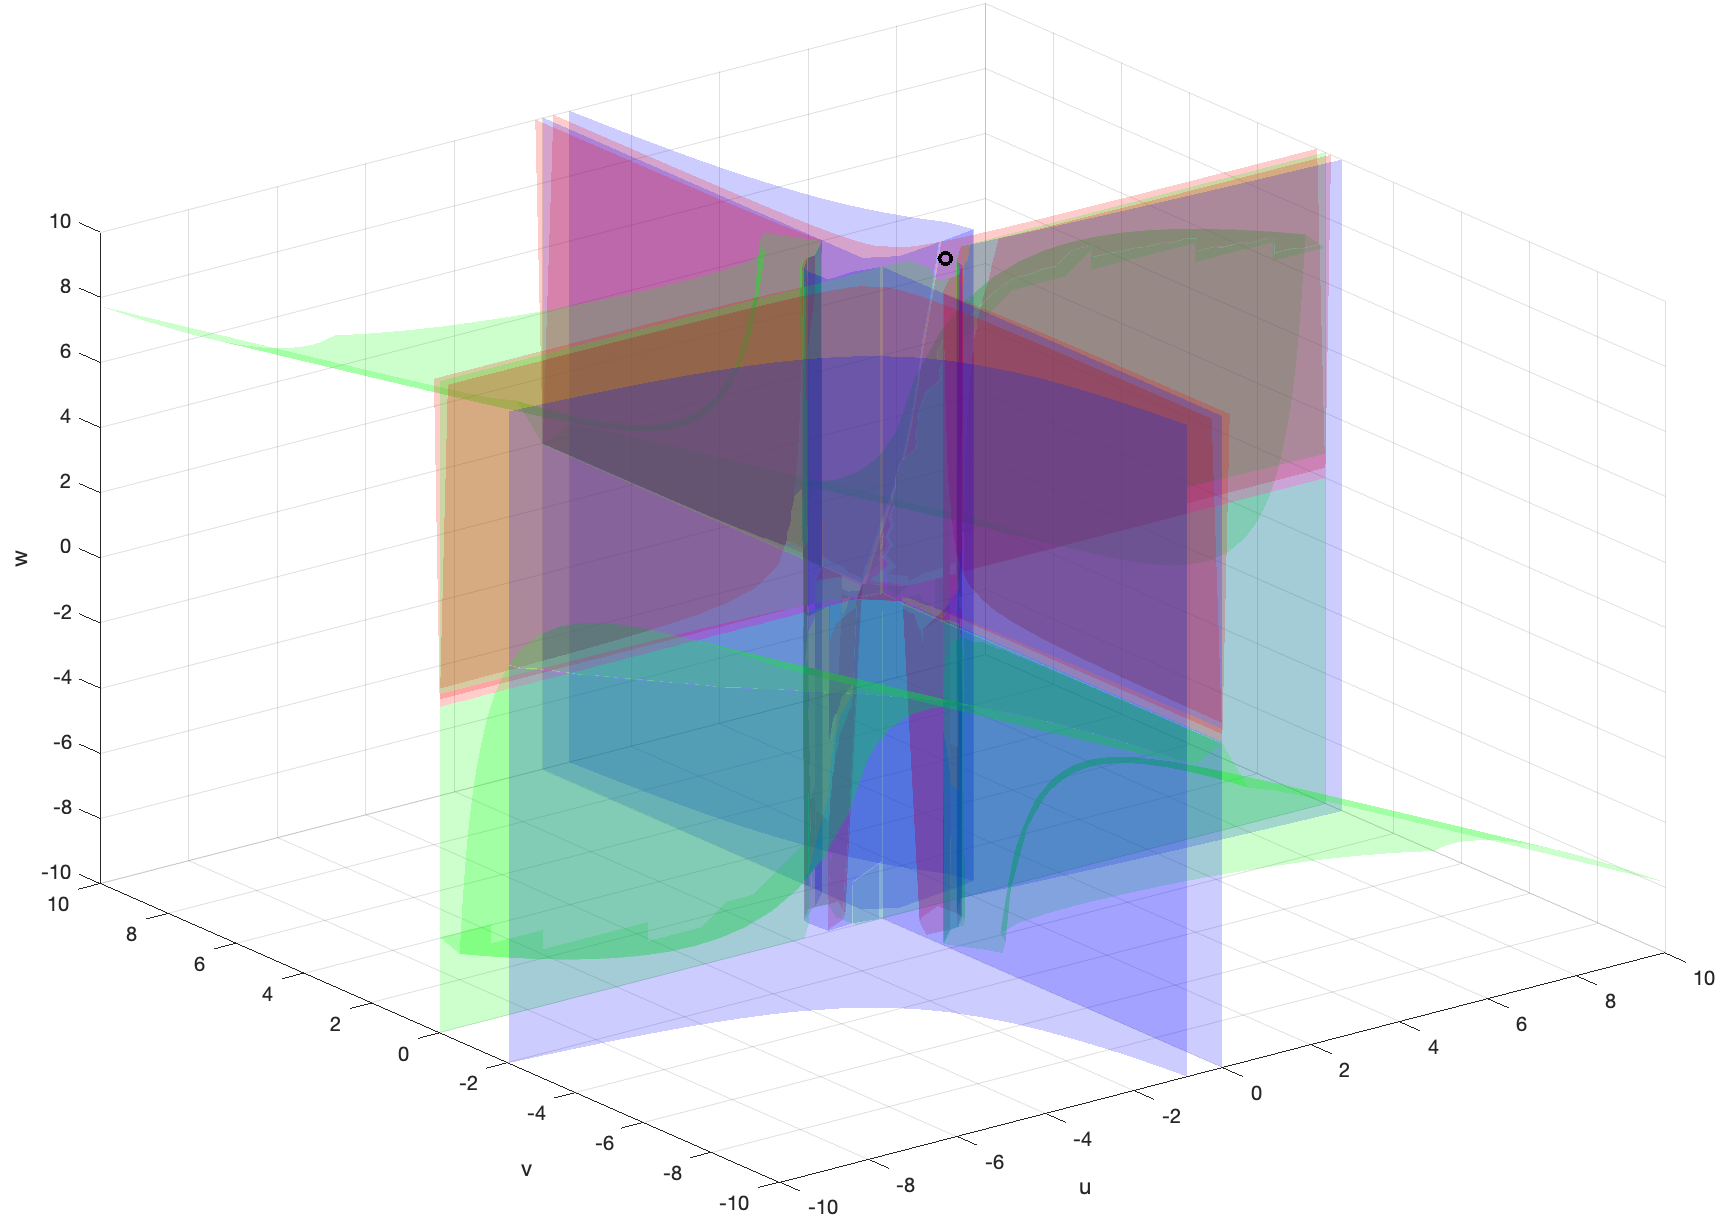
\includegraphics[width=\linewidth]{figures/nullclines.png}}
\end{figure}

\section{Behavior of the system}

Looking at the kinetics system, the Jacobian matrix $A$ is given by $A(\uu, \vv, \ww) = (a_{ij})_{1 \le i, j, \le n}$, with

$$
A(\uu, \vv, \ww) = \bpm  -\mu_f +  \dfrac{m_1\vv}{(1+\uu \vv)^2} - \mu_b \vv &  \dfrac{m_1 \uu}{(1+\uu \vv)^2} - \mu_b \uu & 0 \\[1.2em]
 \dfrac{m_2 \vv}{(1+\uu \vv)^2} - \mu_b \vv   & -\mu_l + \dfrac{m_2 \uu}{(1+\uu \vv)^2} - \mu_b \uu - \ww  & -\vv \\[1.2em] 
  \dfrac{m_3 \vv}{(1+\uu \vv)^2} &  \dfrac{m_3 \vv}{(1+\uu \vv)^2} & -\mu_e \epm
$$
The jacobian can actually be represented in a nicer form. Since we are only interested of value of the jacobian taken at steady states, we can make use of the following identities 

\begin{equation}
	\label{identities}
	 f^1(u, v, w) = 0 \quad\quad f^2(u, v, w) = 0 \quad\quad f^3(u, v, w) = 0
\end{equation}


\subsection{In a neighborhood of the origin}

When taking $(u, v, w) = (0, 0, 0)$, almost all terms in the Jacobian disappear, leaving us with

$$
A(0, 0, 0) = \bpm  -\mu_f  &  0 & 0 \\[1.2em]
0  & -\mu_l & 0 \\[1.2em] 
0 & 0 & -\mu_e \epm
$$

which, by positivity of $\mu_f, \mu_b, \mu_e$ is unconditionally stable. Take a moment to convince yourself that in this case, there is no hope for DDI (to see why, notice that $\tr (A-\bm\mu D) < 0$ and $\det (A-\bm\mu D) = -\mu_f(\mu_l+ \bm\mu / \gamma)(\mu_e + \bm\mu d_2 / \gamma) < 0$ for all non-negative choices of $\bm\mu$). This tells us the system will always be stable, a statement that is corroborated by running a few simulations (see figure \ref{fig:simulations}).

\begin{figure}
	\centering
	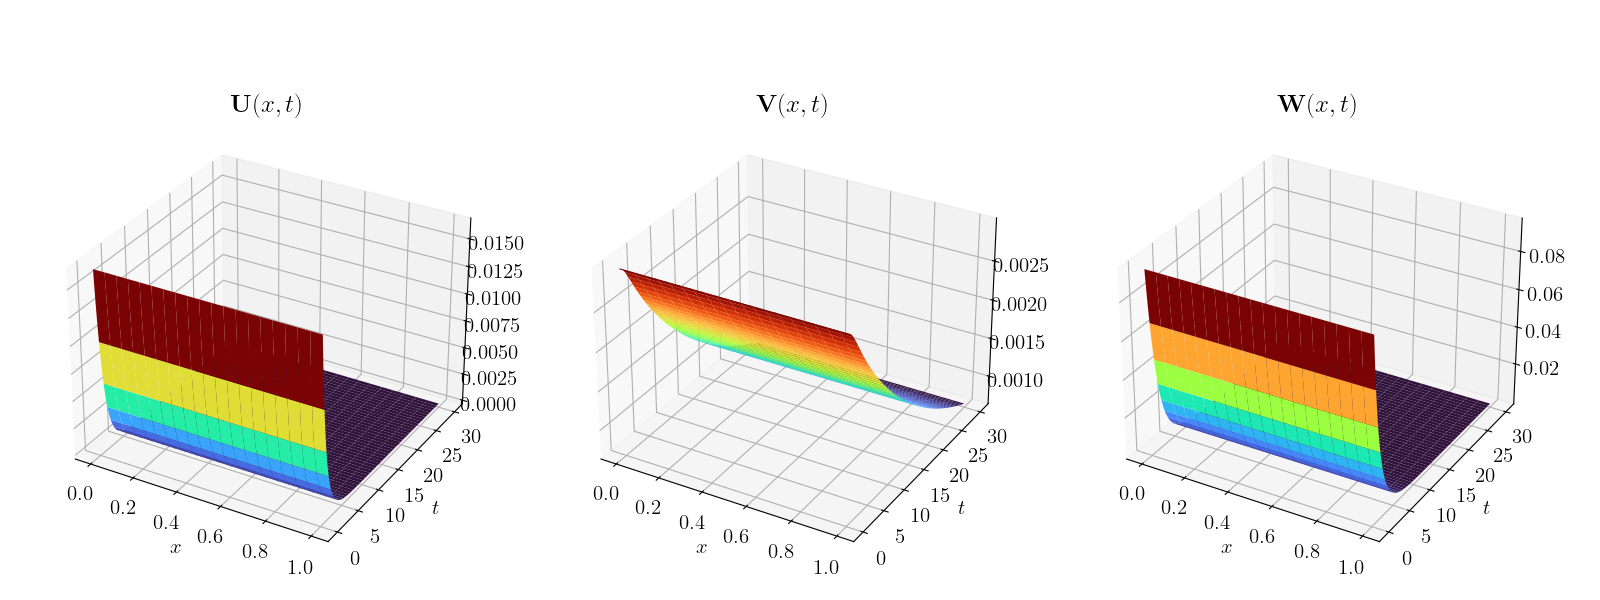
\includegraphics[width=\textwidth]{figures/stable_origin.png}
	\caption{space-time plot of numerical solutions $u, v, w$ to \ref{system} with constant initial condition $\bm X_0 = (\uu_0, \vv_0, \ww_0)$ close to the origin. One clearly sees how each quantity converges towards 0}
	\label{fig:simulations}
\end{figure}

\subsection{Around the other steady state}

Let us move our interest to the other stable steady state (provided the choice of parameters allows it to exist). Using the fact that each term $u, v, w$ is positive, we can operate some surgery on identities \ref{identities} to derive

\begin{equation}
	\label{new_identities}
		m_1 \dfrac{\vv}{1 + \uu \vv} = \mu_f +  \mu_b \vv \quad \quad
		m_2 \dfrac{\uu}{1 +   \uu \vv}  = \mu_l +  \mu_b \uu + \ww \quad \quad
		m_3 \dfrac{ \uu \vv}{1 +  \uu \vv} = \mu_e \ww
\end{equation}
Now notice that by virtually adding '0', we get
$$m_1 \frac{\vv}{(1+\uu\vv)^2} = m_1 \frac{\vv+ \uu\vv^2 - \uu \vv^2}{(1 + \uu\vv)^2} = m_1 \lp\frac{\vv}{1+uv} - \frac{\uu\vv^2}{(1 + \uu\vv)^2}\rp$$
Hence, the coefficient $a_{11}$ of the Jacobian becomes
$$a_{11} = -\mu_f - \mu_b \vv + m_1 \frac{\vv}{1+\uu\vv} - m_1 \frac{\uu\vv^2}{(1 + \uu\vv)^2} \overset{\ref{new_identities}}{=\!=\!=} -m_1 \frac{\uu\vv^2}{(1 + \uu\vv)^2}$$



\begin{theorem}[Routh-Hurwitz criterion of order 3]
	Take a matrix $M \in \euM_3(\R)$. Then all the roots of $\chi_M$ lie in the negative half-plane (i.e. $\sigma(M) \subset \R_{<0}$) if and only if
	$\Delta_i(M) > 0$ for $i=1, 2, 3$ holds, where we define
	\begin{align*}
		\Delta_1(M) &= -\tr(M) \\[0.7em]
		\Delta_2(M) &= -\tr(M) \sum_{i < j} \det(M_{ij}) + \det(M) \\[0.7em]
		\Delta_3(M) &= -\det(M) \Delta_2(M),
	\end{align*}
Alternatively, let $\Tilde{\chi}_{M}(\lambda) = a_0 + a_1 \lambda + a_2 \lambda^2 + \lambda^3$ be the normalized characteristic polynomial of $M$. Then all roots of $\Tilde{\chi}_M$ lie in the negative half-plane if and only if all coefficients are positive and $a_2 a_1 > a_0$.
\end{theorem}


\begin{lemma}[Necessary condition for DDI] Let $B := A - \lambda D$ denote the matrix of the linearized system. We claim that we obtain DDI if and only if $\det(B_{12}) < 0$ and 
	
\end{lemma}


\begin{remark}[Minimum] The function $\mu \longmapsto |A - \mu D|$ reaches its minimum at the point:
	
\begin{equation}
	\resizebox{\hsize}{!}{%
		$\mu_{\mathbf{\mathrm{min}}} = \dfrac{\gamma}{2}\left( \dfrac{1}{(1+uv)^2}\left( m_2 u -  \dfrac{m_1m_2uv + \mu_b^2 uv(1+uv)^4 - \mu_b(m_1 + m_2) uv(1+uv)^2}{m_1 v - \mu_f (1 + uv)^2 - \mu_b v(1+uv)^2} \right)-\dfrac{\mu_e}{d_2} - \mu_l - \mu_b u - w\right) \notag$  
	}
\end{equation}
Please do not make me compute $\det(A - \mu_{\textrm{min}} D)$ ;-;. Also
\begin{equation}
	\resizebox{\hsize}{!}{%
		$\mu_{\mathbf{\mathrm{min}}} > 0 \quad \iff\quad \mu_f \biggl(m_2 - \mu_b u (1 + uv)^2\biggr) > \left( \dfrac{\mu_e}{d_2} + \mu_l + w \right) \biggl( m_1 v - \mu_f(1+uv)^2 - \mu_b v (1 + uv)^2\biggr) \notag$  
	}
\end{equation}
\end{remark}



$$\frac{|A_{12}| + |A_{13}|d_2}{2a_{11} d_2}$$


